\documentclass{article} \usepackage{amsmath} \usepackage{amssymb} \usepackage{amsthm} \usepackage[margin=0.2in]{geometry} \usepackage{hyperref} \usepackage{physics} \usepackage{tikz} \usepackage{mathtools} \mathtoolsset{showonlyrefs} \theoremstyle{definition} \newtheorem{theorem}{Theorem}[section] \newtheorem{corollary}{Corollary}[theorem] \newtheorem{lemma}[theorem]{Lemma} \newtheorem{definition}{Definition}[section] \author{Connor Duncan} \date{\today}
\title{Physics-105-Lecture-Notes-02-28-2019}
\begin{document}
\maketitle\tableofcontents
\noindent\abstract{A single PDF with all lectures in a single document can be downloaded at \url{https://www.dropbox.com/sh/8sqzvxghvbjifco/AAC9LoSRnsRQDp7pYedgWpQMa?dl=0}. The password is 'analytic.mech.dsp'.
 This file was automatically generated using a script, so there might be some errors. If there are, you can contact me at \url{mailto:ctdunc@berkeley.edu}.}
\subsection{Central Force Motion, Continued} Recall, we have $m\ddot r-\frac{l^2}{mr^3}=f(r)$, with constant energy \begin{equation} E=\frac{1}{2}m\dot r^2+\frac{1}{2}\frac{l^2}{mr^2}+V(r)\equiv\text{constant} \end{equation} which allows us to write \begin{align} \dot\theta=\dv{\theta}{t}=\frac{l}{mr^2}\\ d\theta=\frac{ldr}{mr^2\sqrt{\frac{2}{m}\left(E-V(r)-\frac{l^2}{2mr^2}\right)}}\\ \theta=\theta_0+\int_{r_0}^r\frac{dr}{mr^2\sqrt{\frac{2mE}{l^2}-\frac{2mV}{l^2}-\frac{1}{r^2}}}\\ \theta=\theta_0+\int_{u_0}^u\frac{du}{\sqrt{\frac{2mE}{l^2}-\frac{2mV(u)}{l^2}-u^2}} \end{align} If we let $f\sim\frac{1}{r^2}$, we get that, with $k$ as a coupling constant (i.e. how much force is scaled by). \begin{align} \frac{1}{r}=\frac{mk}{l^2}\left(1+\sqrt{1+\frac{2El^2}{mk^2}}\cos(\theta-\theta_0)\right) \end{align} an example of $k$ for gravity is $V=\frac{GmM}{r}$, leaves $k=GmM$. \subsubsection{Kepler Orbits/Phase Diagrams} \begin{align} \frac{1}{r}=c\left(1+\epsilon\cos(\theta-\theta_0)\right)\\ \epsilon=\sqrt{1+\frac{2El^2}{mk^2}}\equiv\text{eccentricity of orbit} \end{align} Now, we want to think about phase diagrams. We have \begin{equation} (\sqrt{E})^2=\left(\frac{p}{\sqrt{2m}}\right)^2+\left(\sqrt{\frac{k}{2}}x\right)^2 \end{equation} So particles move on circles in this abstract phase space \begin{center} 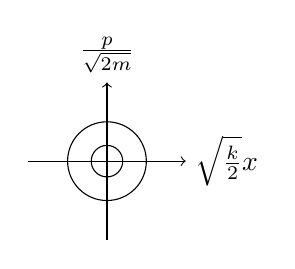
\begin{tikzpicture} \draw[->](-1,0)--(1,0)node[anchor=west]{$\sqrt{\frac{k}{2}}x$}; \draw[->](0,-1)--(0,1)node[anchor=south]{$\frac{p}{\sqrt{2m}}$}; \draw (0,0) ellipse (0.5); \draw (0,0) ellipse (0.2); \end{tikzpicture} \end{center} Recall our diagram of energy from the previous lecture, \begin{center} 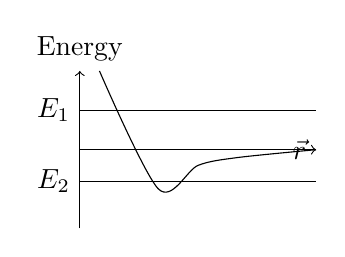
\begin{tikzpicture} \draw[->] (0,-1)--(0,1) node[anchor=south]{Energy}; \draw[->] (0,0)--(3,0) node[anchor=east]{$\vec{r}$}; \draw plot [smooth] coordinates {(0.25,1) (1,-.5) (1.5,-.2) (2,-.1) (3,0) }; \draw (0,.5)node[anchor=east]{$E_1$} --(3,.5); \draw (0,-.4)node[anchor=east]{$E_2$}--(3,-.4); \end{tikzpicture} \end{center} It has a corresponding phase diagram, \begin{center} \begin{tikzpicture} \draw[->] (0,-1)--(0,1) node[anchor=south]{$p$}; \draw[->] (0,0)--(3,0) node[anchor=east]{$\vec{r}$}; \draw (1,0) ellipse (0.3 and 0.1); \end{tikzpicture} \end{center} This is a \emph{suuuuper rough approximation} that you should verify on your own using python or desmos or something. Use $V\sim\frac{1}{r^2}-\frac{s}{r}$ where $s$ is a constant. If curves on the phase diagram are closed, they're \emph{trapped solutions}, i.e. they want to stay within the potential well. For given eccentricity (let $\cos\theta=1$) we can calculate the minimum $r$ of the orbit in a straightforward manner. \begin{equation} r_{min}=\frac{l^2}{mk(1+\epsilon)} \end{equation} and maximum $r$, we have \begin{equation} r_{max}=\frac{l^2}{mk(1-\epsilon)} \end{equation} There are also the unbound orbits, which give you \begin{equation} \frac{1}{r}=C(1+\epsilon\cos(\theta-\theta_0)) \end{equation} the right hand side can be zero, which means $r_{max}\rightarrow\infty$. Let's examine the orbits. First, let $r=\frac{1}{\alpha}(1+\epsilon\cos\theta)$, which gives $\alpha=r+\epsilon r\cos\theta=r+\epsilon x$. Then, we get \begin{itemize} \item $\epsilon=0\rightarrow\frac{1}{r}=\frac{mk}{l^2}$ which gives constant $r$, and is thus a circle. Also note it would give $x^2+y^2=\alpha^2$ which also describes a circle. \item $0<\epsilon<1\rightarrow 0<1+\frac{2El^2}{mk^2}<1\rightarrow \frac{-mk^2}{2l^2}<E<0$. This case corresponds to the area of our energy diagram beneath $E=0$. Completing the square, we alsonote that $\frac{\left(x+\frac{\alpha\epsilon}{1-\epsilon^2}\right)^2}{a^2}+\frac{y^2}{b^2}=1$, where $a=\frac{\alpha}{1-\epsilon^2},b=\frac{\alpha}{\sqrt{1-\epsilon^2}}$. $a$ is called the \emph{semimajor axis}, and $b$ the \emph{semiminor axis}. $\epsilon$ is a unitless quantity. This centers the ellipse at $x_0=-\frac{\alpha\epsilon}{1-\epsilon^2}$. The ellipse also has a \emph{focus}, with $c^2+b^2=a^2$, $c$ being the focus. You can solve it to be $c=\frac{\alpha\epsilon}{1-\epsilon^2}$, and another focus at the origin. \item $\epsilon=1$. We get $y^2=\alpha^2-2\alpha x$, since the $x^2$ terms from our other equation cancel, which gives the parabola $y^2=-2\alpha\left(x-\frac{\alpha}{2}\right)$. \item $\epsilon>1$. We find $\frac{\left(x-\frac{\alpha\epsilon}{\epsilon^2-1}\right)^2}{a^2}-\frac{y^2}{b^2}=1$, which gives a hyperbola! \end{itemize} For a better explanation of what's happening here/pictures, see Taylor fig. 8.11. \subsubsection{Keplers Laws} This lets us derive keplers laws \begin{enumerate} \item Planets Move in ellipses with one focus at the sun (equiv to condition $0\leq\epsilon<1$) \item Radius vector sweeps out equal area at equal time (equiv to conservation of momentum $\dv{A}{t}=\frac{1}{2}r^2\dot\theta=\frac{l}{2m}$. \item The square of the period of an orbit ($T$) is proportional to the cube of the semimajor axis ($T^2=\frac{4\pi^2a^3}{Gm_0}$). This can be shown with $\dv{A}{t}=\frac{l}{2m}\rightarrow A=\frac{l}{2m}T=\pi ab\equiv$area of ellipse. \end{enumerate}
\end{document}
